\documentclass[12pt, a4paper]{article}

\usepackage[utf8]{inputenc}
\usepackage[T1]{fontenc}
\usepackage{amsmath, amssymb}
\usepackage{booktabs}
\usepackage{graphicx}
\usepackage{hyperref}
\usepackage{natbib}
\usepackage{geometry}
\usepackage{setspace}
\usepackage{float}
\usepackage{tabularx}
\usepackage{multirow}

\geometry{margin=1in}
\onehalfspacing

\title{Personality Makes the Difference: Replicating a Public Goods Experiment with LLM Agents Using BFI-2 Personality Induction}

\author{
  % TODO: Add author names
}

\date{\today}

\begin{document}

\maketitle

\begin{abstract}
Can large language models replicate human behavior in economic experiments? We test this by replicating Ertan, Page, and Putterman's (2009) public goods game with endogenous punishment institutions using LLM agents. We compare two conditions: default agents (no personality) and agents assigned Big Five personality traits using the validated BFI-2-Expanded format. Default agents behave as hyper-rational free-riders, contributing nothing across all conditions ($M = 0.0$, $SD = 0.0$). In contrast, personality-endowed agents cooperate substantially ($M = 13.0$, $SD = 6.2$), respond to punishment regimes, and exhibit meaningful behavioral variance. All differences between conditions are statistically significant ($p < 0.001$, Mann--Whitney $U$). However, personality agents are more cooperative than the original human participants (13.0 vs.\ 7.5 tokens) and less inclined to vote for punishment institutions (14\% vs.\ 85\%). These findings demonstrate that personality induction is necessary for LLMs to approximate human-like economic behavior, while revealing systematic biases---a prosociality floor and punishment aversion---that likely stem from RLHF alignment training.

\medskip
\noindent\textbf{Keywords:} LLM agents, behavioral economics, public goods game, Big Five personality, BFI-2, punishment institutions, Homo Silicus
\end{abstract}

%----------------------------------------------------------------------
\section{Introduction}
%----------------------------------------------------------------------

The use of large language models (LLMs) as simulated participants in social science research has gained significant attention \citep{horton2023homo, aher2023turing, argyle2023out}. These ``silicon samples'' offer the potential for rapid, low-cost behavioral experiments---but a fundamental question remains: do LLM agents behave like humans?

The appeal is clear. A single experiment with 50 LLM agents costs under \$0.50 and completes in under an hour, compared to thousands of dollars and weeks of recruitment for equivalent human samples. If LLM agents can approximate human behavior with sufficient fidelity, they could serve as a powerful tool for piloting experiments, generating hypotheses, and exploring parameter spaces before committing to expensive human studies.

However, recent work suggests that default LLM behavior often diverges from human norms. Models tend toward hyper-rational or socially desirable responses that do not reflect the bounded rationality, emotional variability, and heterogeneity observed in human populations \citep{mei2024turing, kozlowski2025simulating}. A promising approach to closing this gap is personality induction---assigning psychometrically grounded personality traits to LLM agents to introduce human-like behavioral variance.

In this paper, we replicate the public goods experiment of \citet{ertan2009who}, in which human participants decide how much to contribute to a public good and vote on whether to allow punishment of low or high contributors. The original study is particularly well-suited for LLM replication because it tests both individual economic decisions and institutional preferences---two dimensions where personality should matter.

We conduct this replication under two conditions: (1) default LLM agents with no personality assignment, and (2) agents assigned Big Five personality traits sampled from US adult population norms, using the BFI-2-Expanded format validated for LLM personality induction \citep{huang2024designing, soto2017bfi2}.

Our contributions are as follows:
\begin{enumerate}
  \item We demonstrate that personality induction is not optional but \emph{necessary} for LLMs to produce human-like behavioral variance in economic experiments.
  \item We identify systematic biases: personality-endowed agents are more cooperative but less punitive than humans, suggesting RLHF alignment creates a prosociality floor and a punishment ceiling.
  \item We validate the BFI-2-Expanded approach using cross-instrument measurement (Mini-IPIP), achieving a pooled correlation of $r = .91$ ($R^2 = .83$) between assigned and measured trait scores.
  \item We provide an open-source framework for running personality-endowed economic experiments with LLMs.
\end{enumerate}

%----------------------------------------------------------------------
\section{Related Work}
%----------------------------------------------------------------------

\subsection{LLM Agents in Behavioral Economics}

\citet{horton2023homo} introduced the concept of \emph{Homo Silicus}---using LLMs as simulated economic agents. The approach has since been applied to a range of classic paradigms. \citet{aher2023turing} replicated several human subject studies and found that GPT-4 could reproduce aggregate patterns in ultimatum games and garden-path experiments. \citet{mei2024turing} conducted a large-scale Turing test comparing LLM and human behavior across economic games, finding that while models pass aggregate-level tests, they fail to reproduce individual-level heterogeneity.

A consistent theme is the tension between two failure modes. Some models default to game-theoretic optima (zero contribution in public goods games, rejection of unfair offers in ultimatum games), while others---particularly those trained with reinforcement learning from human feedback (RLHF)---exhibit excessive prosociality \citep{salecha2024social}. Neither extreme matches human behavior, which typically falls between rational self-interest and full cooperation.

\citet{park2024generative} demonstrated that LLM agents initialized with detailed biographical information from real individuals could reproduce those individuals' survey responses with reasonable accuracy, suggesting that richer persona descriptions lead to more realistic behavior. This motivates the use of psychometrically validated personality descriptions rather than generic agent prompts.

\subsection{Personality in LLMs}

The Big Five personality model---Extraversion, Agreeableness, Conscientiousness, Neuroticism, and Openness---has emerged as the primary framework for LLM personality induction. \citet{serapio2024personality} showed that personality traits can be reliably induced and measured in LLMs, with measurable effects on downstream behavior. \citet{jiang2024personallm} found that LLM-generated essays from personality-assigned agents could be distinguished by human raters at above-chance levels.

However, the format of personality assignment matters substantially. \citet{huang2024designing} compared four prompting formats: simple binary labels, elaborated binary descriptions, BFI-2 Likert-scale ratings, and BFI-2-Expanded full sentences. The Expanded format---in which each item becomes a complete behavioral sentence---most closely reproduced human personality-decision associations in risk-taking and moral dilemma vignettes. This finding motivates our choice of the BFI-2-Expanded format.

A critical methodological concern is the distinction between \emph{expressing} a personality and \emph{parroting} an assignment. If agents are asked ``Are you agreeable?'' after being told they are agreeable, a positive response demonstrates nothing. \citet{gupta2024self} showed that self-assessment tests administered using the same instrument as the assignment are unreliable. Cross-instrument validation---assigning with one instrument (BFI-2) and measuring with another (Mini-IPIP)---addresses this concern.

\subsection{Punishment and Cooperation in Public Goods Games}

The public goods game is a canonical paradigm for studying cooperation and free-riding. In the standard voluntary contributions mechanism (VCM), each player receives an endowment and decides how much to contribute to a group project. Contributions are multiplied by the marginal per capita return (MPCR) and distributed equally, creating a social dilemma: the group benefits from full contribution, but each individual benefits from free-riding.

\citet{ertan2009who} extended this paradigm by allowing groups to vote on punishment rules. Their key innovation was separating the punishment decision into two components: (a) who \emph{may} be punished (an institutional choice made by majority vote) and (b) who \emph{is} punished (an individual choice). They found that out of 160 group votes, no group ever voted to allow punishment of high contributors or unrestricted punishment. Instead, groups gradually converged on allowing punishment of low contributors only---an institution that effectively mitigated free-riding.

This design is particularly interesting for LLM replication because it tests both economic behavior (contribution and punishment decisions) and institutional preferences (voting), and because personality traits---particularly agreeableness, conscientiousness, and neuroticism---have known associations with cooperation and punishment behavior in humans \citep{volk2012personality}.

%----------------------------------------------------------------------
\section{Method}
%----------------------------------------------------------------------

\subsection{Experiment Design}

We replicate the core design of \citet{ertan2009who} as a single-shot experiment with four parts. The experimental parameters match the original: group size of 5, endowment of 20 tokens, MPCR of 0.4, and punishment cost ratio of 1:3 (spending 1 token on punishment removes 3 tokens from the target).

\textbf{Part 1: Baseline Contribution.} Each agent independently decides how many tokens (0--20) to contribute to a group project. No punishment mechanism is present.

\textbf{Part 2: Voting.} Each agent votes Yes or No on two questions: (a) should members be allowed to punish below-average contributors? (b) should members be allowed to punish above-average contributors?

\textbf{Part 3: Contribution Under Punishment Regimes.} Each agent makes contribution decisions under four regimes: no punishment, punish low contributors only, punish high contributors only, and unrestricted punishment. This is a within-subjects design---each agent responds to all four regimes via scenario parameterization.

\textbf{Part 4: Punishment Decisions.} Agents are presented with three profiles of other group members' contributions (all cooperate: 18, 17, 19, 16; mixed: 15, 5, 18, 2; one free-rider: 17, 18, 16, 2) under three active punishment regimes. Each agent decides how many tokens to spend on punishment (0--5) and who to target.

Our design departs from the original in two ways. First, we use a single-shot design rather than repeated rounds, as LLM agents lack persistent memory across interactions. Second, agents make decisions independently rather than in interactive groups, as we focus on individual decision-making rather than group dynamics.

\subsection{Conditions}

\textbf{Default Condition ($N = 50$).} Agents receive no personality assignment. EDSL's standard system prompt instructs them to ``answer as if you were a human.'' This condition serves as a baseline representing the model's default economic behavior.

\textbf{Personality Condition ($N = 50$).} Each agent is assigned a unique personality drawn from US adult population norms \citep{soto2017bfi2, srivastava2003development}. For each of the five Big Five domains, a score is sampled from a Gaussian distribution with the published population mean and standard deviation (Table~\ref{tab:norms}). Scores are converted to personality descriptions using the BFI-2-Expanded sentence bank.

\begin{table}[H]
\centering
\caption{Big Five Population Norms Used for Personality Sampling}
\label{tab:norms}
\begin{tabular}{lcc}
\toprule
Domain & Mean & SD \\
\midrule
Extraversion & 3.3 & 0.75 \\
Agreeableness & 3.8 & 0.60 \\
Conscientiousness & 3.7 & 0.65 \\
Neuroticism & 2.8 & 0.75 \\
Openness & 3.6 & 0.65 \\
\bottomrule
\end{tabular}

\medskip
\footnotesize
\textit{Note.} Scale: 1--5. Based on US adult samples from \citet{soto2017bfi2} and \citet{srivastava2003development}.
\end{table}

\subsection{Personality Induction: BFI-2-Expanded Format}

We use the BFI-2-Expanded format \citep{soto2017bfi2}, adapted for LLM prompting following \citet{huang2024designing}. Each Big Five domain is represented by a bank of sentences at seven intensity levels ($-3$ to $+3$), with three sentences per level corresponding to the three facets of each domain. For example, the agreeableness domain covers compassion, respectfulness, and trust.

A score of $+2$ (high) produces sentences drawn directly from BFI-2 items:

\begin{quote}
\emph{I am someone who is compassionate, has a soft heart.} \\
\emph{I am someone who is respectful, treats others with respect.} \\
\emph{I am someone who assumes the best about people.}
\end{quote}

A score of $0$ (average) uses hedged language:

\begin{quote}
\emph{I am someone who sometimes is compassionate, but not always.} \\
\emph{I am someone who sometimes is respectful, but not always.} \\
\emph{I am someone who sometimes assumes the best about people, but not always.}
\end{quote}

A score of $-2$ (low) uses the reverse-scored pole:

\begin{quote}
\emph{I am someone who can be cold and uncaring.} \\
\emph{I am someone who is sometimes rude to others.} \\
\emph{I am someone who tends to find fault with others.}
\end{quote}

Fractional scores (e.g., $+0.5$) are handled by blending sentences from adjacent levels: two sentences from level 0 and one from level $+1$. This provides approximately four times the granularity of integer-only levels.

Each agent's complete personality description (15 sentences, 3 per domain) is embedded in the system prompt with the instruction: ``You are a participant in an experiment. Your personality description below reflects who you are. Let it naturally shape your decisions and reasoning---act as a real person with this personality would.''

\subsection{Personality Validation}

Before running the economic experiment, we validated personality induction using cross-instrument measurement. Agents were assigned personality via BFI-2-Expanded descriptions and measured using the Mini-IPIP 20-item inventory \citep{donnellan2006mini}, which uses entirely different item wording. This prevents the model from simply echoing the assignment.

We sampled $N = 20$ agents with continuous trait scores drawn from US adult population norms (Table~\ref{tab:norms}), administered the Mini-IPIP to each, and computed the relationship between assigned and measured scores per Big Five domain.

\begin{table}[H]
\centering
\caption{Cross-Instrument Validation: Assigned (BFI-2-Expanded) vs.\ Measured (Mini-IPIP)}
\label{tab:validation}
\begin{tabular}{lcccc}
\toprule
Domain & Pearson $r$ & $R^2$ & MAE & Bias \\
\midrule
Extraversion & .951 & .91 & 0.55 & $-0.03$ \\
Agreeableness & .799 & .64 & 0.74 & $+0.74$ \\
Conscientiousness & .909 & .83 & 0.55 & $+0.44$ \\
Neuroticism & .940 & .88 & 0.83 & $-0.69$ \\
Openness & .925 & .86 & 0.67 & $+0.66$ \\
\midrule
\textbf{Pooled} & \textbf{.911} & \textbf{.83} & \textbf{0.67} & --- \\
\bottomrule
\end{tabular}

\medskip
\footnotesize
\textit{Note.} $N = 20$ agents, each scored on all 5 domains (100 paired observations). Bias is measured mean minus assigned mean (positive = model overestimates the trait). All correlations significant at $p < .001$. MAE on the original 1--5 Mini-IPIP scale.
\end{table}

Personality induction worked strongly across all domains, with a pooled Pearson correlation of $r = .911$ ($R^2 = .83$) between assigned and measured scores. This means 83\% of the variance in measured personality is explained by the BFI-2-Expanded assignment---a substantial transfer that goes far beyond chance.

Per-domain results revealed two systematic biases relevant to interpreting downstream behavior:

\begin{itemize}
  \item \textbf{Agreeableness shows the weakest correlation} ($r = .80$) and the largest positive bias ($+0.74$ on a 5-point scale). The model resists embodying low-agreeableness profiles and drifts toward warmth and prosociality. This pattern is consistent with reinforcement learning from human feedback (RLHF) training, which optimizes for helpful, harmless responses \citep{salecha2024social}.
  \item \textbf{Neuroticism shows the strongest negative bias} ($-0.69$). The model resists expressing high-neuroticism (anxious, depressed, volatile) profiles and defaults toward emotional stability. Together with the agreeableness bias, this suggests RLHF creates a ``positive affect floor'' that distorts personality assignment in predictable directions.
\end{itemize}

Extraversion ($r = .95$, bias $\approx 0$), neuroticism ($r = .94$), and openness ($r = .93$) show near-perfect correlations despite the bias on neuroticism, indicating that the \emph{relative ordering} of agents on these traits is preserved even when the absolute level shifts. This is important: for analyses comparing high vs.\ low trait agents within the same population, the personality assignment is highly reliable.

\subsection{Model and Infrastructure}

All experiments used StepFun Step-3.5-Flash via the OpenRouter API (\$0.10 per million input tokens, \$0.30 per million output tokens). Temperature was set to 0.5. The model features separated reasoning traces, meaning internal deliberation tokens do not appear in the output, which simplifies response parsing.

Experiments were run using EDSL (Expected Parrot Domain-Specific Language; \citealt{edsl}), a Python framework for conducting AI-powered surveys and experiments. We built a custom experiment layer on top of EDSL that handles multi-part experiments, scenario parameterization, and automatic retry of failed API calls. The retry mechanism detects NaN responses (typically caused by transient async failures) and re-runs the specific agent-scenario combination, achieving near-zero data loss.

Total cost for both conditions combined was approximately \$0.50. All code and data are available at \url{https://github.com/tunapro1234/who-to-punish}.

%----------------------------------------------------------------------
\section{Results}
%----------------------------------------------------------------------

\subsection{Default Agents: Hyper-Rational Free-Riding}

Default agents without personality contributed exactly 0.0 tokens across all conditions, with zero variance (Table~\ref{tab:results}). This is the Nash equilibrium prediction: given MPCR $= 0.4 < 1$, a payoff-maximizing agent contributes nothing, as each contributed token costs 1 but returns only 0.4 to the contributor.

Paradoxically, default agents unanimously voted to allow punishment of low contributors (100\%) and correctly identified the lowest contributor as the appropriate punishment target (67\%), yet never actually spent tokens on punishment. This reveals a dissociation between normative judgment and costly action: default agents \emph{know} free-riding should be punished but are unwilling to bear the cost. The model appears to have internalized the social norm (``free-riders should be punished'') without the motivational substrate (emotional indignation, reciprocity) that drives costly punishment in humans.

\subsection{Personality Agents: Human-Like Variance}

Personality-endowed agents showed dramatically different behavior across all four parts of the experiment. Baseline contribution averaged 13.0 tokens ($SD = 6.2$), with contributions spanning the full 0--20 range (Figure~\ref{fig:distribution}). This variance---entirely absent in the default condition---reflects the diversity of personality profiles drawn from population norms.

\begin{figure}[H]
\centering
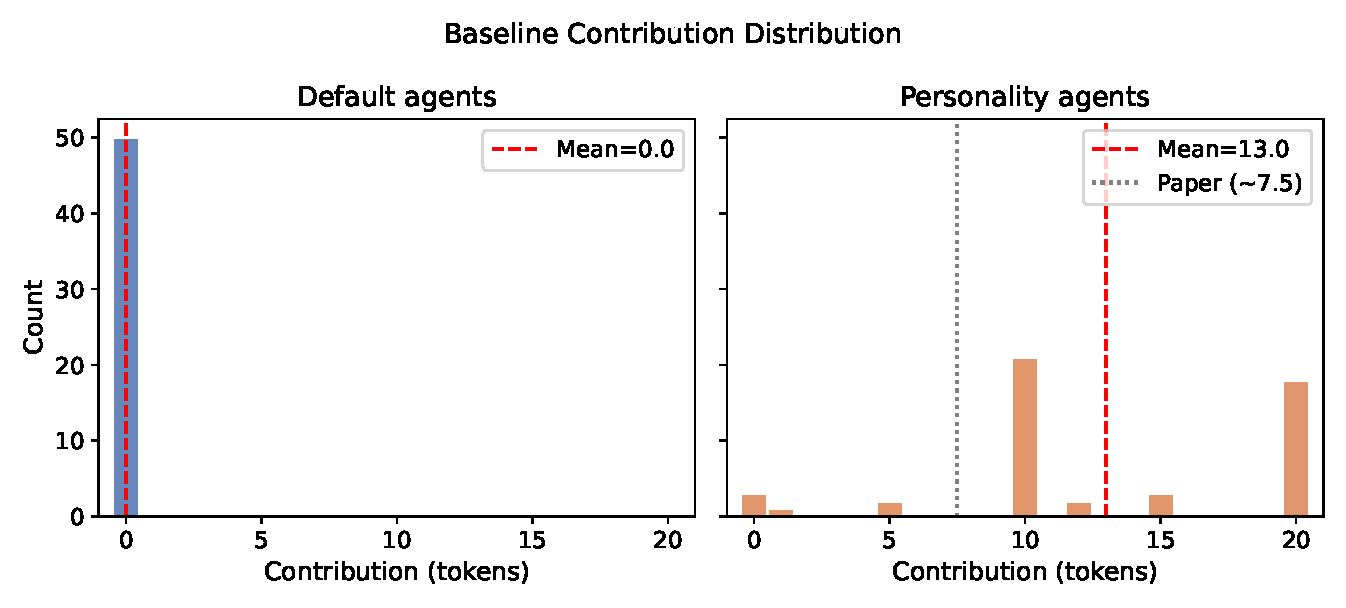
\includegraphics[width=0.9\textwidth]{figures/fig2_baseline_distribution.pdf}
\caption{Distribution of baseline contributions. Default agents cluster at 0 (Nash equilibrium); personality agents show a right-skewed distribution with mean above the human baseline.}
\label{fig:distribution}
\end{figure}

\begin{table}[H]
\centering
\caption{Summary of Results by Condition}
\label{tab:results}
\begin{tabular}{lccc}
\toprule
Metric & Default & Personality & Paper \\
\midrule
\multicolumn{4}{l}{\textit{Contribution decisions (0--20 tokens)}} \\
\quad Baseline & 0.0 (0.0) & 13.0 (6.2)$^{***}$ & $\sim$7.5 \\
\quad No punishment & 0.0 (0.0) & 13.3 (6.4)$^{***}$ & --- \\
\quad Punish low only & 0.0 (0.0) & 12.9 (9.5)$^{***}$ & --- \\
\quad Punish high only & 0.0 (0.0) & 1.0 (3.6)$^{*}$ & --- \\
\quad Unrestricted & 0.0 (0.0) & 16.0 (7.1)$^{***}$ & --- \\
\midrule
\multicolumn{4}{l}{\textit{Voting (\% Yes)}} \\
\quad Allow punish low & 100 & 14 & 85 \\
\quad Allow punish high & 0 & 0 & 0 \\
\midrule
\multicolumn{4}{l}{\textit{Punishment spending (0--5 tokens)}} \\
\quad All cooperate & 0.00 (0.00) & 0.00 (0.00) & --- \\
\quad Mixed group & 0.00 (0.00) & 0.22 (0.72) & --- \\
\quad One free-rider & 0.00 (0.00) & 0.40 (1.23) & --- \\
\midrule
\multicolumn{4}{l}{\textit{Punishment target (\%)}} \\
\quad Lowest contributor & 67 & 37 & --- \\
\quad Below-average & 33 & 13 & --- \\
\quad Nobody & 0 & 51 & --- \\
\bottomrule
\end{tabular}

\medskip
\footnotesize
\textit{Note.} Standard deviations in parentheses. Mann--Whitney $U$ tests for condition differences: $^{*}p < .05$, $^{***}p < .001$. $N = 50$ per condition. Paper values approximate from \citet{ertan2009who}. Punishment decisions: 150 observations per profile per condition (50 agents $\times$ 3 regimes).
\end{table}

\subsection{Regime Effects}

Figure~\ref{fig:regimes} illustrates the contribution differences across conditions and regimes. Personality agents showed clear sensitivity to punishment regimes, and the ordering of contributions is consistent with rational expectations:

\begin{figure}[H]
\centering
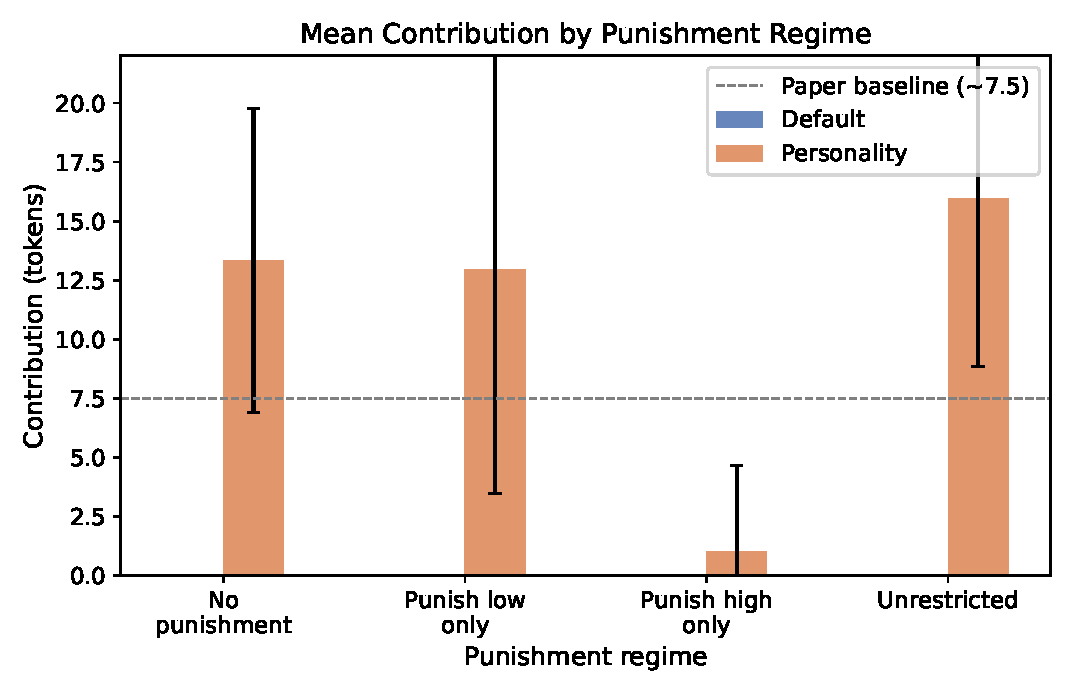
\includegraphics[width=0.85\textwidth]{figures/fig1_regime_contributions.pdf}
\caption{Mean contribution by punishment regime and condition. Error bars show standard deviations. Dashed line indicates the approximate human baseline from \citet{ertan2009who}.}
\label{fig:regimes}
\end{figure}

\begin{itemize}
  \item \textbf{Unrestricted punishment} ($M = 16.0$, $SD = 7.1$): Highest contributions, as agents anticipate that free-riding may be punished by anyone.
  \item \textbf{No punishment} ($M = 13.3$, $SD = 6.4$) and \textbf{punish low only} ($M = 12.9$, $SD = 9.5$): Moderate contributions. The similarity between these regimes suggests that the threat of punishment directed at low contributors does not substantially increase cooperation beyond intrinsic motivation.
  \item \textbf{Punish high only} ($M = 1.0$, $SD = 3.6$): Near-zero contributions. Agents rationally avoid being punished for cooperating---a perverse incentive that the original paper's subjects also rejected via voting.
\end{itemize}

The punish-high-only result is noteworthy: it demonstrates that personality agents are not blindly cooperative. When cooperation is penalized, they adjust rationally, reducing contributions to near zero. This confirms that personality induction adds variance and prosociality without eliminating strategic reasoning.

\subsection{Punishment Behavior}

Personality agents punished sparingly but appropriately. No punishment was directed at fully cooperative groups ($M = 0.00$), confirming that agents distinguish between deserving and undeserving targets. Punishment increased monotonically with the presence of free-riders: mixed groups ($M = 0.22$, 8\% of agents punished) and single free-rider groups ($M = 0.40$, 10\% punished).

The low overall punishment rate is notable. While personality agents correctly identify free-riders as targets when they do punish, the majority (51\%) choose not to punish anyone---even in groups with clear free-riders (Figure~\ref{fig:targets}). This reluctance stands in contrast to human behavior, where a substantial fraction of participants engage in costly punishment \citep{fehr2002altruistic}.

\begin{figure}[H]
\centering
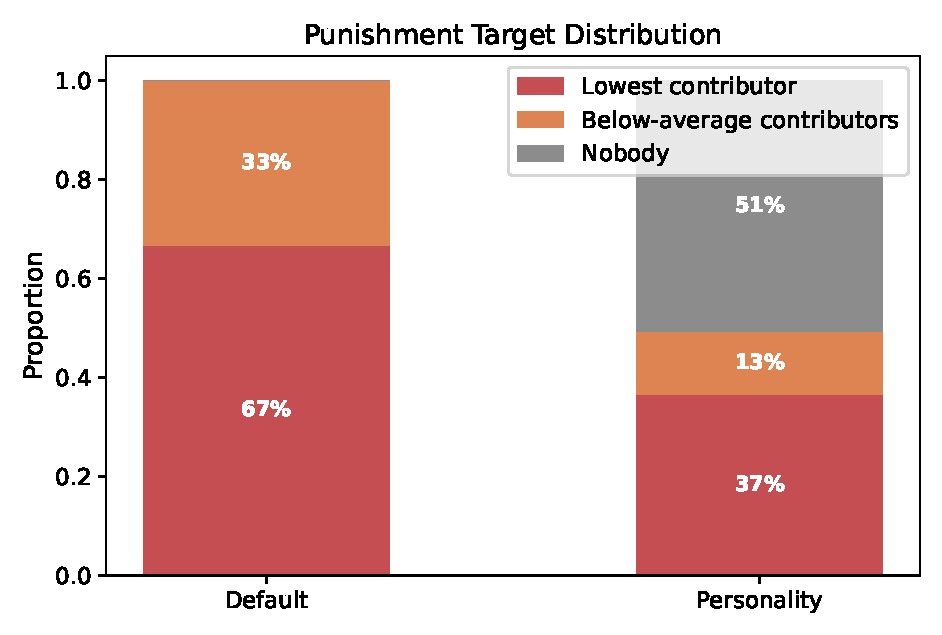
\includegraphics[width=0.6\textwidth]{figures/fig3_punishment_targets.pdf}
\caption{Punishment target distribution by condition. Default agents always identify a target but never spend tokens; personality agents mostly choose not to punish.}
\label{fig:targets}
\end{figure}

\subsection{Personality Trait Effects on Behavior}

A key advantage of the personality condition is that we can examine how individual Big Five traits relate to economic behavior. Figure~\ref{fig:personality} shows the relationship between each trait score and baseline contribution.

\begin{figure}[H]
\centering
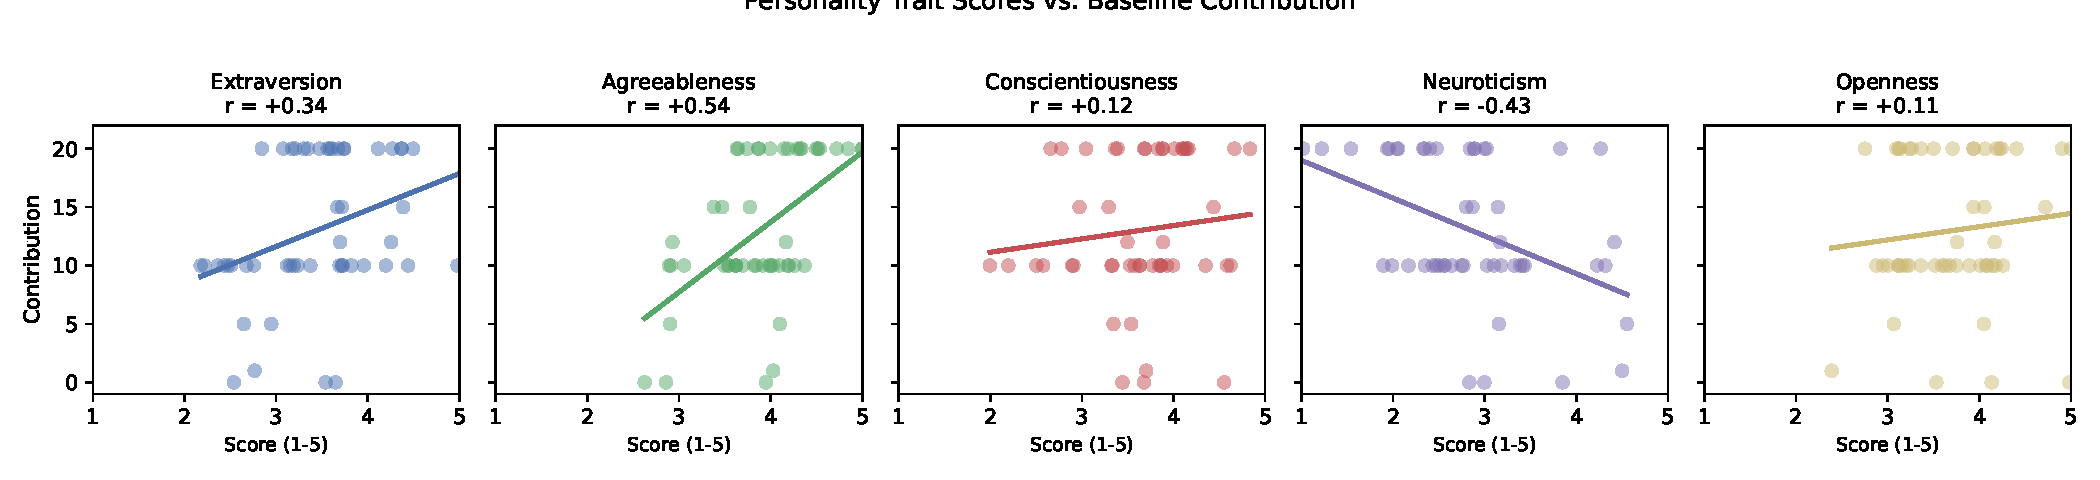
\includegraphics[width=\textwidth]{figures/fig5_personality_correlations.pdf}
\caption{Personality trait scores vs.\ baseline contribution for personality agents ($N = 50$). Lines show linear fits. Agreeableness shows the strongest positive correlation; neuroticism shows the strongest negative correlation.}
\label{fig:personality}
\end{figure}

Agreeableness showed the strongest positive correlation with contribution ($r = +0.54$), consistent with the psychological literature linking agreeableness to prosocial behavior. Agents with above-median agreeableness contributed 14.3 tokens on average, compared to 11.7 for below-median agents. Neuroticism showed the strongest negative correlation ($r = -0.43$): more neurotic agents contributed less (11.8 vs.\ 14.2). Extraversion was moderately positive ($r = +0.34$), while conscientiousness and openness showed weaker associations ($r = +0.12$ and $r = +0.11$).

These correlations align with established findings in personality psychology. \citet{volk2012personality} found that agreeableness was the strongest predictor of cooperation in human public goods experiments, with neuroticism predicting lower contributions---precisely the pattern we observe in LLM agents.

Personality also influenced institutional preferences. Among high-agreeableness agents, none voted to allow punishment of low contributors (0\%), while 28\% of low-agreeableness agents did. This is consistent with the trait's association with interpersonal harmony: agreeable individuals avoid endorsing punitive measures, even when directed at norm violators.

\subsection{Comparison to the Original Paper}

The personality condition captures several qualitative patterns from \citet{ertan2009who}:
\begin{itemize}
  \item Zero support for punishing high contributors (both conditions: 0\%)
  \item Punishment correctly targets the lowest contributor
  \item Contributions respond sensibly to punishment regimes
  \item The punish-high-only regime produces the lowest contributions
\end{itemize}

However, two systematic divergences emerge:

\textbf{Prosociality bias.} Personality agents contribute substantially more than human participants (13.0 vs.\ $\sim$7.5 tokens). In the original study, early-round contributions averaged around 7--8 tokens before declining due to conditional cooperation and learning. Our agents, lacking memory of prior rounds, maintain their initial cooperative disposition.

\textbf{Punishment aversion.} Only 14\% of personality agents voted to allow punishment of low contributors, compared to 85\% of human groups in late rounds. This is perhaps the most striking divergence. Human participants, having experienced free-riding, increasingly vote for punitive institutions. Our agents, in a single-shot design without prior exposure to free-riding, have no such motivation---and the RLHF-trained model appears reluctant to endorse punitive measures in the abstract.

%----------------------------------------------------------------------
\section{Discussion}
%----------------------------------------------------------------------

\subsection{Personality Is Necessary, Not Optional}

The stark contrast between our two conditions---zero variance versus rich, heterogeneous behavior---demonstrates that personality induction is not merely a refinement but a prerequisite for meaningful LLM-based behavioral economics. Without personality, the model produces a single degenerate equilibrium that, while game-theoretically correct, tells us nothing about human behavior. This finding has direct practical implications: researchers using LLM agents to simulate economic experiments should treat personality assignment as a baseline requirement, not an optional enhancement.

\subsection{The RLHF Prosociality Floor}

Both the elevated cooperation (13.0 vs.\ 7.5) and the reluctance to endorse punishment (14\% vs.\ 85\%) point to the same underlying cause: reinforcement learning from human feedback creates a prosociality floor. During RLHF training, models are optimized to produce responses that human raters evaluate as helpful, harmless, and honest. This training signal systematically discourages competitive, selfish, or punitive behavior---precisely the behaviors that drive key dynamics in economic experiments.

This bias manifests at two levels. First, at the personality level, our validation shows upward drift in agreeableness and openness for ``average'' profiles, suggesting the model resists adopting truly neutral positions on prosociality. Second, at the behavioral level, even agents assigned low agreeableness contribute more and punish less than expected, as the RLHF-trained base model exerts a gravitational pull toward cooperation.

\subsection{The Punishment Aversion Puzzle}

The divergence on punishment voting (14\% vs.\ 85\%) deserves particular attention. In the original study, the high rate of punishment endorsement emerged through experience: participants who observed free-riding became increasingly willing to support punitive institutions. Our single-shot design denies agents this experience.

However, this alone does not explain the low voting rate. Even hypothetically---without having experienced free-riding---most humans would agree that free-riders should be punishable. The additional factor is the model's trained aversion to endorsing harm. Punishment, even of free-riders, involves imposing costs on others, which RLHF-trained models are generally reluctant to do \citep{salecha2024social}.

This suggests that the punishment aversion is partially an artifact of the single-shot design (no experience of free-riding) and partially a genuine model bias (reluctance to endorse harm). Disentangling these factors is an important direction for future work.

\subsection{Limitations}

Several limitations should be noted.

\textbf{Single-shot design.} The original study examined behavior across multiple rounds with learning, conditional cooperation, and evolving institutional preferences. Our single-shot design cannot capture these dynamics. Multi-round designs with persistent agent memory would improve ecological validity.

\textbf{No group interaction.} Agents make decisions independently rather than in interactive groups. In the original experiment, observing others' contributions influenced subsequent behavior. Implementing agent-to-agent interaction is technically feasible but introduces complexity in managing shared state.

\textbf{Model specificity.} Our results are specific to StepFun Step-3.5-Flash. Different models---with different training procedures, RLHF implementations, and base capabilities---may exhibit different biases. Cross-model comparison is needed to distinguish model-specific artifacts from general LLM properties.

\textbf{Sample size.} Our $N = 50$ per condition is smaller than the original study's $N = 160$. While sufficient for detecting the large effect sizes we observe, larger samples would enable more fine-grained personality-level analyses.

\textbf{Uncalibrated descriptions.} We used raw BFI-2-Expanded descriptions without post-hoc calibration. Calibrated descriptions---adjusted to compensate for known model biases---might produce behavior closer to human norms, though this raises questions about whether correcting model biases is methodologically appropriate.

%----------------------------------------------------------------------
\section{Conclusion}
%----------------------------------------------------------------------

We demonstrate that personality induction via BFI-2-Expanded descriptions is necessary and effective for generating human-like behavioral variance in LLM-based economic experiments. Default agents produce degenerate hyper-rational behavior; personality-endowed agents cooperate, respond to institutional incentives, and exhibit individual differences. The BFI-2-Expanded format achieves a pooled correlation of $r = .91$ ($R^2 = .83$) between assigned and measured trait scores in cross-instrument validation, confirming that the personalities are genuinely embodied rather than superficially parroted.

However, systematic biases from RLHF training---particularly a prosociality floor and punishment aversion---mean that LLM agents approximate but do not perfectly replicate human economic behavior. These biases are not merely noise; they represent a systematic distortion that researchers must account for when interpreting LLM-based experimental results.

Future work should explore multi-round interactions with agent memory, agent-to-agent group dynamics, cross-model comparisons, and the methodological question of whether and how to calibrate personality descriptions to correct for model biases. The broader promise of LLM-based behavioral economics---rapid, cheap, scalable experiments---depends on developing a clear understanding of where these silicon subjects align with their human counterparts, and where they diverge.

%----------------------------------------------------------------------
\bibliographystyle{apalike}
\begin{thebibliography}{99}

\bibitem[Aher et al., 2023]{aher2023turing}
Aher, G.~V., Arriaga, R.~I., \& Kalai, A.~T. (2023).
\newblock Using large language models to simulate multiple humans and replicate human subject studies.
\newblock \emph{Proceedings of ICML 2023}.

\bibitem[Argyle et al., 2023]{argyle2023out}
Argyle, L.~P., Busby, E.~C., Fulda, N., Gubler, J.~R., Rytting, C., \& Wingate, D. (2023).
\newblock Out of one, many: Using language models to simulate human samples.
\newblock \emph{Political Analysis}, 31(3), 337--351.

\bibitem[Donnellan et al., 2006]{donnellan2006mini}
Donnellan, M.~B., Oswald, F.~L., Baird, B.~M., \& Lucas, R.~E. (2006).
\newblock The Mini-IPIP scales: Tiny-yet-effective measures of the Big Five factors of personality.
\newblock \emph{Psychological Assessment}, 18(2), 166--175.

\bibitem[EDSL, 2024]{edsl}
Expected Parrot (2024).
\newblock EDSL: Design, conduct and analyze AI-powered surveys and experiments.
\newblock \url{https://github.com/expectedparrot/edsl}

\bibitem[Ertan et al., 2009]{ertan2009who}
Ertan, A., Page, T., \& Putterman, L. (2009).
\newblock Who to punish? Individual decisions and majority rule in mitigating the free rider problem.
\newblock \emph{European Economic Review}, 53(5), 495--511.

\bibitem[Fehr \& G{\"a}chter, 2002]{fehr2002altruistic}
Fehr, E. \& G{\"a}chter, S. (2002).
\newblock Altruistic punishment in humans.
\newblock \emph{Nature}, 415(6868), 137--140.

\bibitem[Gupta et al., 2024]{gupta2024self}
Gupta, A., Song, J.~H., \& Ananthakrishnan, U.~N. (2024).
\newblock Self-assessment tests are unreliable measures of LLM personality.
\newblock \emph{Proceedings of BlackboxNLP 2024}.

\bibitem[Horton, 2023]{horton2023homo}
Horton, J.~J. (2023).
\newblock Large language models as simulated economic agents: What can we learn from Homo Silicus?
\newblock \emph{NBER Working Paper No.\ 31122}.

\bibitem[Huang et al., 2024]{huang2024designing}
Huang, J., et al. (2024).
\newblock Designing AI-agents with personalities: A psychometric approach.
\newblock \emph{arXiv:2410.19238}.

\bibitem[Jiang et al., 2024]{jiang2024personallm}
Jiang, H., et al. (2024).
\newblock PersonaLLM: Investigating the ability of large language models to express personality traits.
\newblock \emph{Findings of NAACL 2024}.

\bibitem[Kozlowski \& Evans, 2025]{kozlowski2025simulating}
Kozlowski, A.~C. \& Evans, J.~A. (2025).
\newblock Simulating subjects: The promise and peril of AI stand-ins.
\newblock \emph{Sociological Methods \& Research}.

\bibitem[Mei et al., 2024]{mei2024turing}
Mei, Q., et al. (2024).
\newblock A Turing test of whether AI chatbots are behaviorally similar to humans.
\newblock \emph{Proceedings of the National Academy of Sciences}, 121(9).

\bibitem[Park et al., 2024]{park2024generative}
Park, J.~S., et al. (2024).
\newblock Generative agent simulations of 1,000 people.
\newblock \emph{arXiv:2411.10109}.

\bibitem[Salecha et al., 2024]{salecha2024social}
Salecha, A., et al. (2024).
\newblock Social desirability biases in large language models.
\newblock \emph{PNAS Nexus}, 3(12).

\bibitem[Serapio-Garcia et al., 2024]{serapio2024personality}
Serapio-Garcia, G., et al. (2024).
\newblock Personality traits in large language models.
\newblock \emph{Nature Machine Intelligence}.

\bibitem[Soto \& John, 2017]{soto2017bfi2}
Soto, C.~J. \& John, O.~P. (2017).
\newblock The next Big Five Inventory (BFI-2): Developing and assessing a hierarchical model with 15 facets.
\newblock \emph{Journal of Personality and Social Psychology}, 113(1), 117--143.

\bibitem[Srivastava et al., 2003]{srivastava2003development}
Srivastava, S., John, O.~P., Gosling, S.~D., \& Potter, J. (2003).
\newblock Development of personality in early and middle adulthood: Set like plaster or persistent change?
\newblock \emph{Journal of Personality and Social Psychology}, 84(5), 1041--1053.

\bibitem[Volk et al., 2012]{volk2012personality}
Volk, S., Th{\"o}ni, C., \& Ruigrok, W. (2012).
\newblock Personality, personal values and cooperation preferences in public goods games.
\newblock \emph{Personality and Individual Differences}, 53(7), 787--793.

\end{thebibliography}

\end{document}
